\section{Data and Experimental Setup}
\label{sec:data_and_experimental_setup}

\subsection{Dataset}
\label{subsec:dataset}
Experiments were performed on the PASCAL VOC 2012 dataset~\cite{dataset_pascal_voc}, which comprises 20 object classes plus one background category. In line with standard practice, the training set was expanded using additional images from the Semantic Boundaries Dataset (SBD)~\cite{sbd_dataset}, yielding a total of 10,582 training images. The original VOC 2012 split contains 1,464 training images, 1,449 validation images, and 1,456 test images. As the ground-truth labels for the test set are not publicly accessible, all evaluations of model performance were carried out on the validation set.

\subsection{Experimental Setup}
\label{subsec:experimental_setup}
All experiments were implemented using the \textbf{PyTorch} framework and executed on a single \textbf{NVIDIA Tesla T4 GPU} with \textbf{16 GB memory}, accessed through Google Colab (free tier).

During training, the input images were randomly resized within the range of 512 to 2048 pixels, rescaled by factors between 0.5 and 2.0, and then cropped to a fixed resolution of $224 \times 224$.

Model optimization was performed using the \textbf{AdamW} optimizer with a learning rate of $5 \times 10^{-5}$, momentum parameters $\beta_1 = 0.9$, $\beta_2 = 0.999$, and a weight decay of 0.01. Training was run for \textbf{30,000 iterations} with an effective batch size of 8 (per-GPU batch size of 4, with gradient accumulation over 2 steps). A linear learning rate warmup was applied for the first 500 iterations, with a warmup ratio of $10^{-3}$. The best model checkpoints were selected based on validation set performance.

\begin{figure}[t]
    \centering
    \fbox{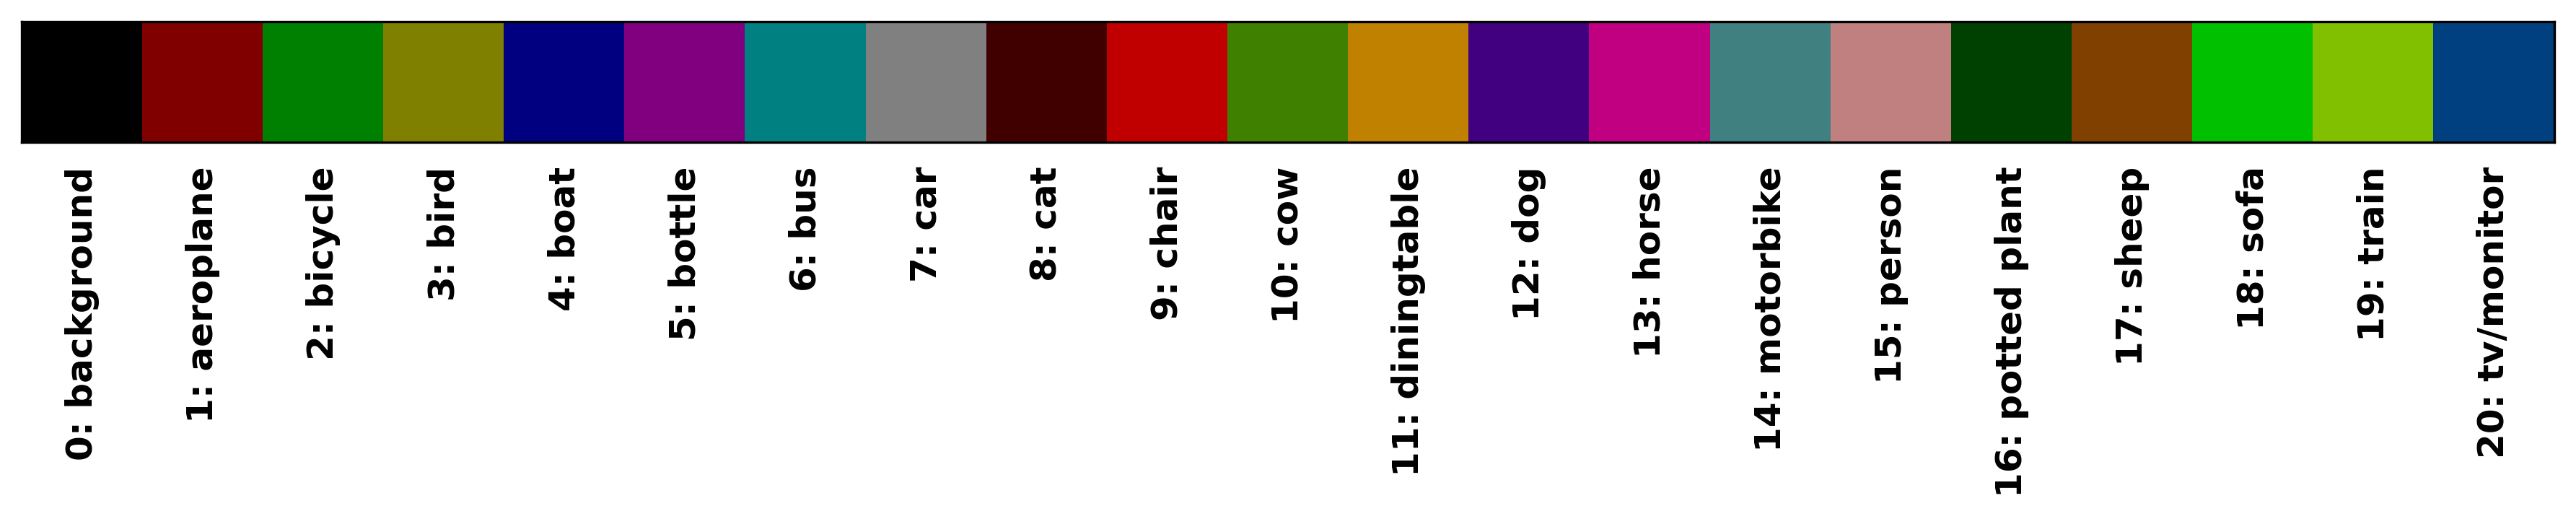
\includegraphics[width=0.98\textwidth]{figures/voc_colormap.png}}
    \caption{Pascal VOC 2012 class color map for visualization. Each class is represented by a unique color for easy identification in segmentation maps.}
    \label{fig:class_colors_voc2012}
\end{figure}

\subsection{Evaluation Metric}
\label{subsec:evaluation_metric}
The primary evaluation criterion was the \textbf{mean Intersection over Union (mIoU)}. For a given class $c$, the Intersection over Union (IoU) is defined as:

$$
\text{IoU}(c) = \frac{TP_c}{TP_c + FP_c + FN_c}
$$

where $TP_c$, $FP_c$, and $FN_c$ denote the number of true positives, false positives, and false negatives for class $c$, respectively. The mean IoU is then computed as the average IoU across all $K$ semantic classes:

$$
\text{mIoU} = \frac{1}{K} \sum_{c=1}^{K} \text{IoU}(c)
$$

This metric is widely used in semantic segmentation as it provides a balanced assessment of model performance across both frequent and infrequent classes.
